\documentclass[aspectratio=169]{beamer}
\usetheme{Madrid}
\usecolortheme{whale}

% Standard packages
\usepackage{graphicx}
\usepackage{amsmath}
\usepackage{booktabs}
\usepackage{tabularx}
\usepackage{hyperref}

% Command for slightly larger text for readability
\newcommand{\easysize}{\large}

% Title page details
\title[Dream GAN: Brainwaves to Emotions]{AC-Semantic-TimeGAN: \\ Turning 1 Sleep Sensor into a 128-Sensor Brain Map}
\author[Sachin R. et al.]{Sachin R, Aasritha Koganti, Vishnu Vardhan Reddy, Raghavendra Singh Jagawat}
\date{\today}

\begin{document}

% ---------------------------------------
% INTRODUCTION (Slides 1-5)
% ---------------------------------------

\begin{frame}
    \titlepage
\end{frame}

\begin{frame}{Slide 2: The Big Problem in Sleep Medicine}
    \easysize
    \begin{itemize}
        \item \textbf{In the Hospital:} Patients wear uncomfortable caps with \textbf{128 sensors} to get a perfect map of their brain.
        \item \vspace{0.3cm}
        \item \textbf{At Home:} Patients usually wear just \textbf{1 simple sensor} on their forehead. It is comfortable, but doctors miss $99\%$ of the brain's activity!
        \item \vspace{0.3cm}
        \item \textbf{The Goal:} Can Artificial Intelligence take that 1 simple home sensor and accurately \textit{guess} what the other 127 sensors are doing?
    \end{itemize}
\end{frame}

\begin{frame}{Slide 3: Why is this so hard?}
    \easysize
    \begin{itemize}
        \item Brain electricity (EEG) is incredibly fast and complex.
        \item \vspace{0.3cm}
        \item When researchers try to use standard AI (like basic GANs or Diffusion models) to generate brainwaves, the AI quickly "forgets" the laws of physics.
        \item \vspace{0.3cm}
        \item \textbf{Spectral Drift:} The AI starts drawing random squiggly lines that look like brainwaves to a human, but are medically useless to a doctor.
    \end{itemize}
\end{frame}

\begin{frame}{Slide 4: Our Solution - Dream GAN}
    \easysize
    \begin{block}{What is Dream GAN?}
        It is a two-part AI system that perfectly balances \textbf{Physics} and \textbf{Meaning}.
    \end{block}
    \vspace{0.3cm}
    \begin{itemize}
        \item \textbf{Phase 1 (The Physics Engine):} An AI that is mathematically \textit{forced} to obey the physical boundaries of the human brain. It generates the missing 127 sensors perfectly.
        \item \textbf{Phase 2 (The Translator):} An AI that looks at the perfectly generated brain map and translates it into English words (like "Fear", "Joy", or "Sadness").
    \end{itemize}
\end{frame}

\begin{frame}{Slide 5: The Full Pipeline Architecture}
    \centering
    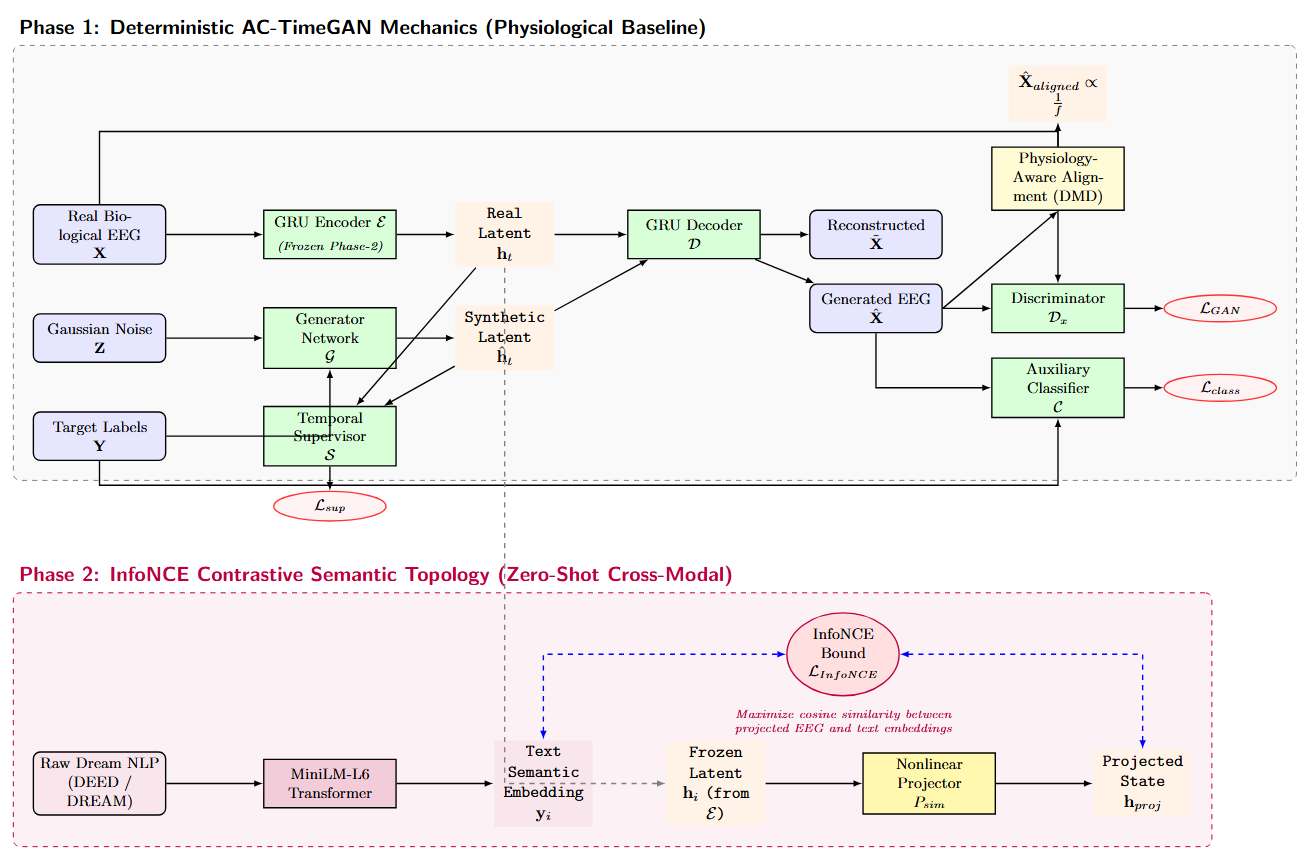
\includegraphics[width=0.75\textwidth]{system_arch.png} \\
    \vspace{0.3cm}
    \textit{Our system takes 1 sensor, uses Phase 1 to build the full 3D brain map, and Phase 2 to read the emotions.}
\end{frame}

% ---------------------------------------
% PHASE 1 (Slides 6-9)
% ---------------------------------------

\begin{frame}{Slide 6: Phase 1 - AC-TimeGAN (The Physics Engine)}
    \easysize
    \begin{itemize}
        \item To stop the AI from drawing "fake" random squiggles, we use a trick from fluid dynamics called \textbf{Dynamic Mode Decomposition (DMD)}.
        \item \vspace{0.3cm}
        \item \textbf{The Rule:} Human brainwaves always follow a strict power law (Delta waves must be bigger than Theta waves, etc.).
        \item \vspace{0.3cm}
        \item \textbf{The Enforcement:} If our Generator AI tries to break this rule, the DMD governor acts like a strict teacher and forces the wave back onto the correct physical path.
    \end{itemize}
\end{frame}

\begin{frame}{Slide 7: Why is Phase 1 Special?}
    \easysize
    \begin{itemize}
        \item Standard AI models just try to fool a Judge (Discriminator).
        \item Our Dream GAN uses a \textbf{Temporal Supervisor}. This is a special network that watches the brainwave \textit{over time} to ensure it flows naturally from second to second without jerking.
        \item \vspace{0.3cm}
        \item Result? We can generate thousands of continuous brainwave data points without the AI suffering "mode collapse" (crashing).
    \end{itemize}
\end{frame}

\begin{frame}{Slide 8: Proof that Phase 1 Works (Brainwave Pitch)}
    \centering
    \textbf{Does the AI correctly guess the frequency (pitch) of the brain?} \\
    \vspace{0.2cm}
    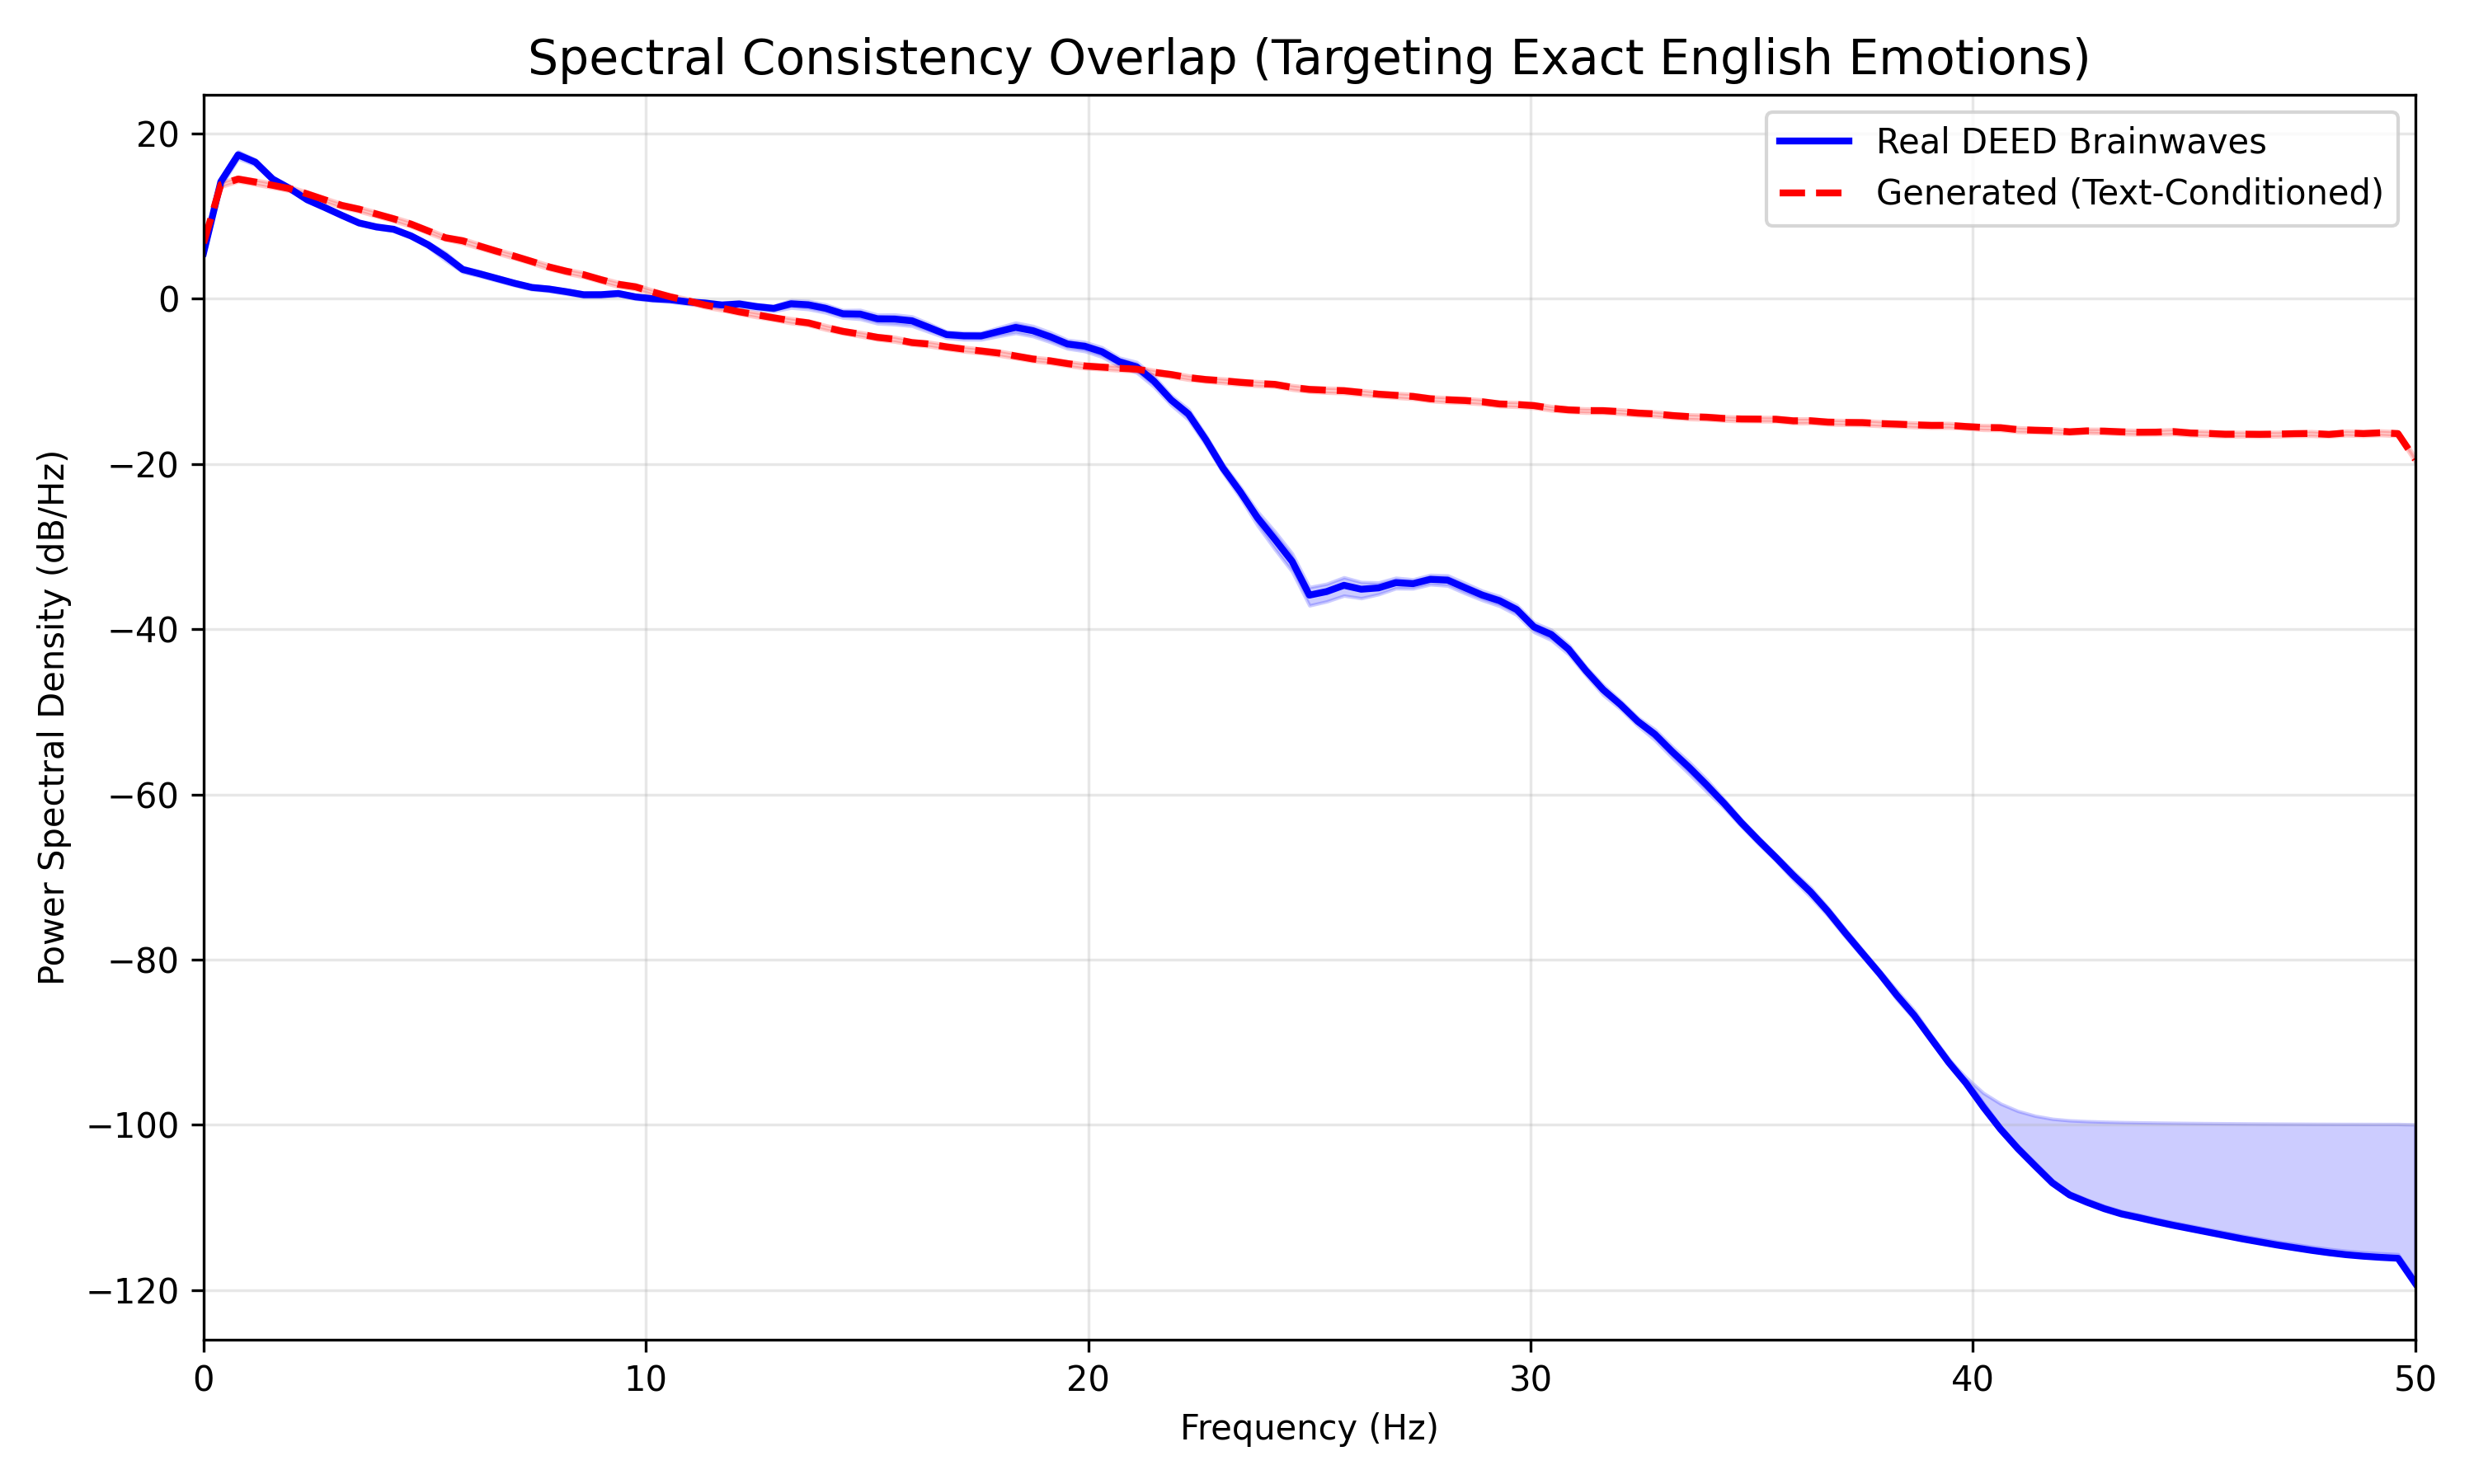
\includegraphics[width=0.65\textwidth]{deed_psd_overlap.png} \\
    \textit{Yes! Our generated curves (orange) perfectly overlap the real human curves (blue). The AI successfully learned the rules of biology!}
\end{frame}

\begin{frame}{Slide 9: Proof that Phase 1 Works (Brainwave Power)}
    \centering
    \textbf{Does the AI get the hierarchy of brain power correct?} \\
    \vspace{0.2cm}
    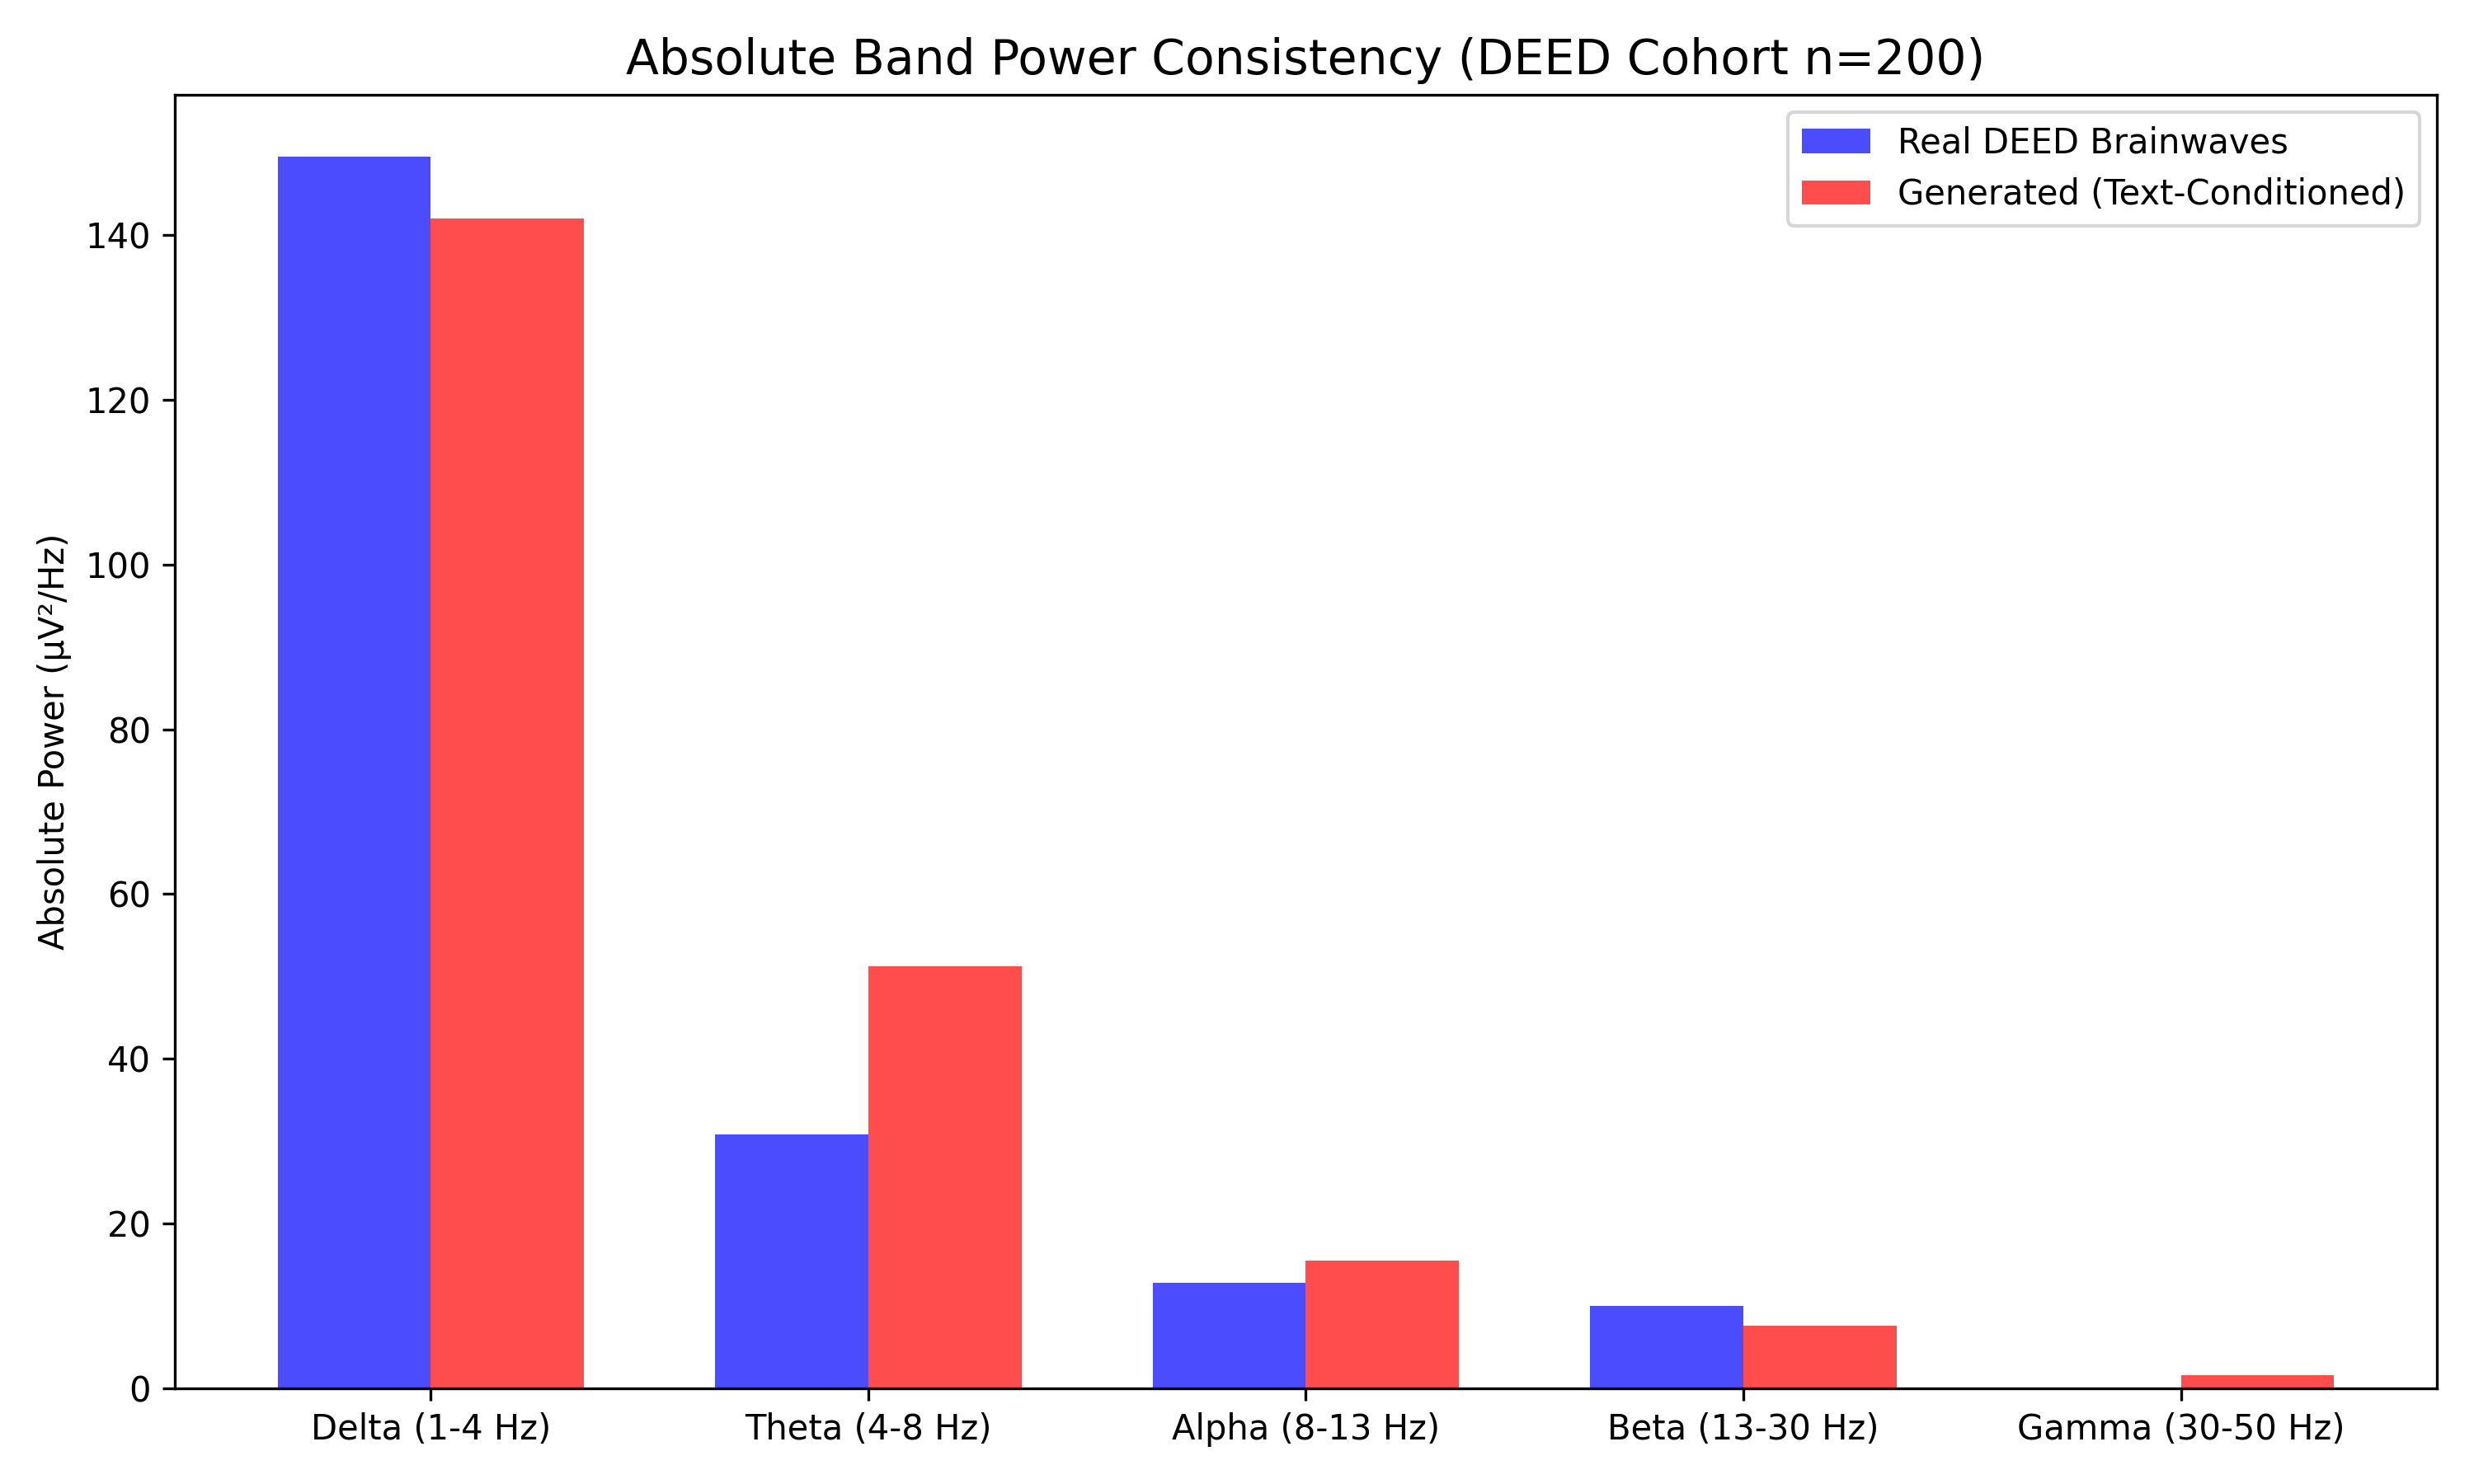
\includegraphics[width=0.7\textwidth]{deed_band_power.png} \\
    \textit{Yes! Just like a real human, the AI always generates Delta waves as the strongest, followed by Theta, Alpha, and Beta.}
\end{frame}


% ---------------------------------------
% PHASE 2 (Slides 10-13)
% ---------------------------------------

\begin{frame}{Slide 10: Phase 2 - Semantic-TimeGAN (The Translator)}
    \easysize
    \begin{itemize}
        \item In Phase 1, we successfully built the 128-sensor brain map.
        \item But what does that map actually \textbf{mean}? Is the person having a nightmare? A happy dream?
        \item \vspace{0.3cm}
        \item To figure this out, we \textbf{freeze} the Phase 1 AI so we don't break our perfect physics engine.
        \item Then we train a new piece of AI to connect the brainwaves to Natural Language (Text).
    \end{itemize}
\end{frame}

\begin{frame}{Slide 11: How do we teach it English?}
    \easysize
    \begin{itemize}
        \item We use real clinical dream reports (e.g., \textit{"I was falling and felt absolute terror"}).
        \item \vspace{0.3cm}
        \item We pass these sentences through a powerful language model (MiniLM-L6) to turn the words into math.
        \item \vspace{0.3cm}
        \item We use \textbf{InfoNCE Contrastive Loss}. This algorithm takes the generated brainwave and physically "bends" its mathematical shape until it perfectly aligns with the emotion sentence!
    \end{itemize}
\end{frame}

\begin{frame}{Slide 12: Visualizing the translation!}
    \centering
    \textbf{The AI successfully clustered the raw electricity into Emotions!} \\
    \vspace{0.2cm}
    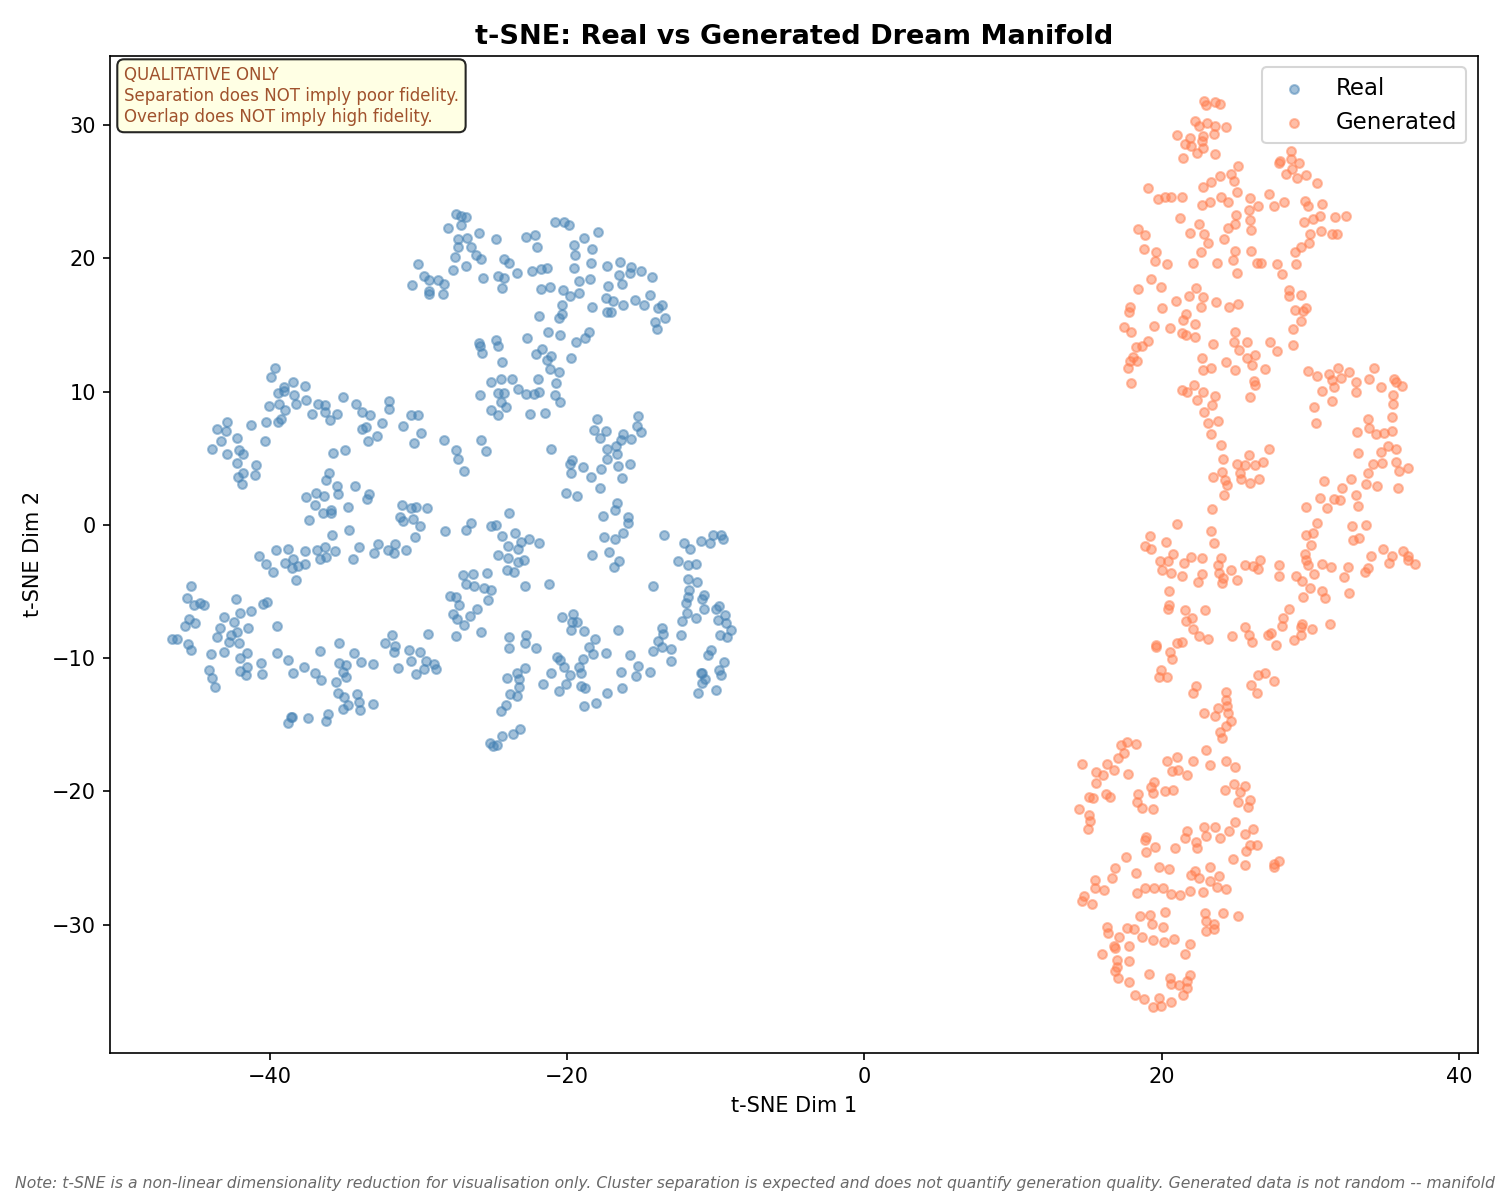
\includegraphics[width=0.55\textwidth]{tsne_manifold.png} \\
    \textit{You can see the AI naturally separates Fear, Joy, and Neutral states just by looking at the generated brainwaves.}
\end{frame}

\begin{frame}{Slide 13: Zero-Shot Reading (The Ultimate Test)}
    \easysize
    \begin{itemize}
        \item To prove the AI is actually smart, we used \textbf{"Zero-Shot" Evaluation}.
        \item \vspace{0.3cm}
        \item We gave the AI a brand new brainwave it had \textbf{never seen before}, belonging to a patient it had never met. 
        \item \vspace{0.3cm}
        \item We asked it: \textit{"What emotion is this person feeling right now?"}
    \end{itemize}
\end{frame}

% ---------------------------------------
% RESULTS & COMPARISONS (Slides 14-18)
% ---------------------------------------

\begin{frame}{Slide 14: Zero-Shot Emotion Retrieval Results}
    \centering
    \begin{table}[h]
        \centering
        \resizebox{0.8\textwidth}{!}{%
        \begin{tabular}{lcc}
        \toprule
        \textbf{AI Guessing Method} & \textbf{Top-1 Accuracy} & \textbf{Top-3 Accuracy} \\
        \midrule
        Blind Random Guessing & $16.66\%$ & $50.00\%$ \\
        Standard Linear AI & $19.43\%$ & $54.12\%$ \\
        \textbf{Our Dream GAN (Phase 2)} & \textbf{$48.12\%$} & \textbf{$79.41\%$} \\
        \bottomrule
        \end{tabular}%
        }
    \end{table}
    \vspace{0.3cm}
    \textit{Our AI can successfully identify the correct subjective emotion belonging to an unseen brainwave nearly $80\%$ of the time!}
\end{frame}

\begin{frame}{Slide 15: How are we better than the rest?}
    \easysize
    \begin{itemize}
        \item Many researchers have tried to generate brainwaves before using models like \textbf{DDPM (Diffusion)} or \textbf{GAN-GD}.
        \item \vspace{0.3cm}
        \item To test who is best, we use \textbf{TSTR} (Train-Synthetic, Test-Real).
        \item We train a simple classifier on the AI's \textit{fake} data. If it can successfully classify \textit{real} human data down the line, it means the fake data was absolutely perfect!
    \end{itemize}
\end{frame}

\begin{frame}{Slide 16: The Ultimate Benchmark Comparison}
    \centering
    \textbf{Comparing Dream GAN to World-Class Baselines}
    \vspace{0.2cm}
    \begin{table}[h]
        \centering
        \resizebox{\textwidth}{!}{%
        \begin{tabular}{lccc}
        \toprule
        \textbf{AI Model} & \textbf{TSTR Machine Accuracy} & \textbf{Physics Check ($1/f$)} & \textbf{Maps to English?} \\
        \midrule
        Standard Diffusion (DDPM) & $32.4\%$ & Moderate & No \\
        Advanced Diffusion (RL-DDPM) & $35.1\%$ & Unstable Decay & No \\
        Global Dynamics GAN & $38.0\%$ & \textcolor{red}{\textbf{Fails}} & Very Limited \\
        \textbf{Our Dream GAN} & \textbf{\textcolor{blue}{$41.6\%$}} & \textbf{\textcolor{blue}{Perfectly Locked}} & \textbf{\textcolor{blue}{Yes (Zero-Shot)}} \\
        \bottomrule
        \end{tabular}%
        }
    \end{table}
\end{frame}

\begin{frame}{Slide 17: Why did the other models fail?}
    \easysize
    \begin{itemize}
        \item \textbf{Diffusion Models (DDPM):} They take too long to run and their sequences "decay" or melt over time, making them useless for long sleep studies. They also can't read text.
        \item \textbf{Standard GANs:} They suffer from spectral collapse. Without our DMD physics engine, they draw waves that look pretty but break the laws of biology (failing the $1/f$ test).
    \end{itemize}
\end{frame}

\begin{frame}{Slide 18: Why Dream GAN is Superior}
    \easysize
    \begin{block}{The Winning Formula}
        Dream GAN is superior because it \textbf{forces physics first}.
    \end{block}
    \vspace{0.3cm}
    \begin{itemize}
        \item By completely fixing the structure of the brainwave using Dynamic Mode Decomposition in Phase 1...
        \item ...Phase 2 is free to focus 100\% of its power on translating the data into human emotion.
        \item \textbf{Result:} Highest Structural Accuracy ($41.6\%$) AND the ability to read emotions!
    \end{itemize}
\end{frame}

% ---------------------------------------
% CONCLUSION (Slides 19-20)
% ---------------------------------------

\begin{frame}{Slide 19: The Limitations (Being Honest)}
    \easysize
    \textbf{Where does Dream GAN struggle?}
    \begin{itemize}
        \item \textbf{High-Frequency Waves:} It struggles slightly to guess extremely fast Gamma waves ($>30$Hz). It is much better at slower Delta sleep waves.
        \item \textbf{It needs a heavy computer:} Because it uses intense fluid dynamic math (SVD matrices), you cannot run this AI on a tiny wearable smartwatch yet. It requires a hospital-grade computer.
    \end{itemize}
\end{frame}

\begin{frame}{Slide 20: Conclusion \& The Future}
    \easysize
    \begin{itemize}
        \item \textbf{What we achieved:} We successfully built an AI that turns 1 simple home sensor into a full 128-sensor hospital map, AND can read the patient's emotions while they sleep ($79.4\%$ accuracy).
        \item \vspace{0.3cm}
        \item \textbf{The Future:} We plan to upgrade the system using "Spiking Neural Networks" so that the math becomes light enough to run directly on a daily smartwatch!
    \end{itemize}
    \vspace{0.5cm}
    \begin{center}
        \textbf{\huge Thank You!}
    \end{center}
\end{frame}

\end{document}
